\documentclass{article}
\usepackage{graphicx}
\usepackage{subcaption}
\usepackage[margin=2.5cm]{geometry}
\usepackage{breakcites}
\usepackage{indentfirst}
\usepackage{pgfgantt}
\usepackage{pdflscape}
\usepackage{float}
\usepackage{epsfig}
\usepackage{epstopdf}
\usepackage[cmex10]{amsmath}
\usepackage{stfloats}
\usepackage{multirow}

\graphicspath{{./images/}}

\begin{document}

\begin{titlepage}
\begin{center}
\textbf{}\\
\textbf{\Large{ISTANBUL TECHNICAL UNIVERSITY}}\\
\vspace{0.5cm}
\textbf{\Large{COMPUTER ENGINEERING DEPARTMENT}}\\
\vspace{2cm}
\textbf{\Large{BLG 242E\\ DIGITAL CIRCUITS LABORATORY\\ HOMEWORK REPORT}}\\
\vspace{2.8cm}
\begin{table}[ht]
\centering
\Large{
\begin{tabular}{lcl}
\textbf{EXPERIMENT NO}  & : & 3 \\
\textbf{LAB SESSION}  & : & FRIDAY - 16.30 \\
\textbf{GROUP NO}  & : & 18 \\
\end{tabular}}
\end{table}
\vspace{1cm}
\textbf{\Large{GROUP MEMBERS:}}\\
\begin{table}[ht]
\centering
\Large{
\begin{tabular}{rcl}
150200916  & : & Denıs Iurıe Davıdoglu \\
150220770  & : & Onur Baylam \\
\end{tabular}}
\end{table}
\vspace{2.8cm}
\textbf{\Large{SPRING 2023}}

\end{center}

\end{titlepage}
\thispagestyle{empty}
\addtocontents{toc}{\contentsline {section}{\numberline {}FRONT COVER}{}}
\addtocontents{toc}{\contentsline {section}{\numberline {}CONTENTS}{}}
\setcounter{tocdepth}{4}
\tableofcontents
\clearpage

\setcounter{page}{1}

\section{INTRODUCTION}
In this experiment, we implemented logic circuits for arithmetic operations on signed and unsigned binary numbers. Starting with the basic unit, a half-adder, it is extended to a full-adder to allow connections in chains by means of carry ports. Instead of actually building and connecting four full-adders, a dedicated integrated circuit is used to test our knowledge of binary addition and subtraction on real silicon.

\section{MATERIALS AND METHODS}

\subsection{Preliminary}
Signed and unsigned addition for binary numbers in 2's complement notation is done in the same way, with regular long addition, except the only digits available are zero and one, and there is a carry whenever a two or three is obtained. Suppose there are two $n$-bit numbers. Then, if they are regarded as unsigned, every bit's position corresponds to a power of two, and its decimal representation is obtained by calculating the weighted sum of all bits. The least significant bit has a weight of $+2^0$, and the most significant bit has a weight of $+2^{n-1}$. In the case of signed numbers, the most significant bit represent the sign, and in conversion it has a weight of $-2^{n-1}$, while all other bits are interpreted the same. \\

To subtract signed or unsigned binary numbers, 2's complement technique gets involved. Basically, the subtrahend is complemented and incremented by one, which is its 2's complement equivalent. Afterwards, the two numbers are added instead of being subtracted. The result can be converted to decimal as in the case of addition, depending on whether the numbers where signed or unsigned.\\

Carry occurs in unsigned addition and is the $n+1^{th}$ bit. If this bit is zero, there is no carry; and if it is one, there is a carry. When there is a carry, it means that the result of addition does not fit into $n$ bits. Borrow is similar but occurs in unsigned subtraction. If the $n+1^{th}$ bit is zero, there is a borrow; and if it is one, no borrow. Borrow indicates that the result of subtraction cannot be represented with unsigned numbers with $n$ bits. Overflow can occur in signed operations with 2's complement notation whenever the signs of operands and of result become meaningless. If positive added with positive gives negative, if negative subtracted from positive gives negative, if negative added with negative gives positive or if positive subtracted from negative gives positive, there is an overflow.\\ 

To observe all of these, $74xx83$ Four-Bit Binary Full Adder is used in the end of experiment, which allows both addition and subtraction on two four-bit numbers.

\newpage

\subsection{Experiment}

\subsubsection{Experiment - Part 1}
A half adder has two inputs and two outputs, whose behaviour is described by the truth table in Fig. 1a. It is realized using one XOR gate and one AND gate, as in Fig. 1b. During the experiment, this circuit was implemented with 74000 series integrated circuits according to the diagram in Fig. 1c:

\begin{figure}[H]
\begin{subfigure}{0.5\textwidth}
\centering
\begin{tabular}{|c|c|c|c|}
\hline
A & B & SUM & C \\
\hline
0 & 0 & 0 & 0 \\
0 & 1 & 1 & 0 \\
1 & 0 & 1 & 0 \\
1 & 1 & 0 & 1 \\
\hline
\end{tabular}
\subcaption{Truth table}
\end{subfigure}%
\begin{subfigure}{0.5\textwidth}
	\centering
	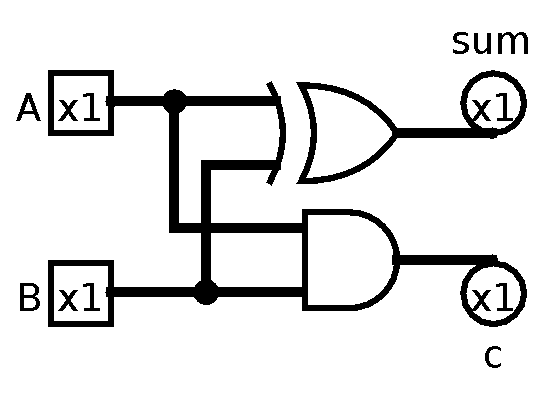
\includegraphics[width=0.7\textwidth]{half_adder_logisim.png}
	\subcaption{Design in Logisim}
\end{subfigure}
\begin{subfigure}{\textwidth}
	\centering
	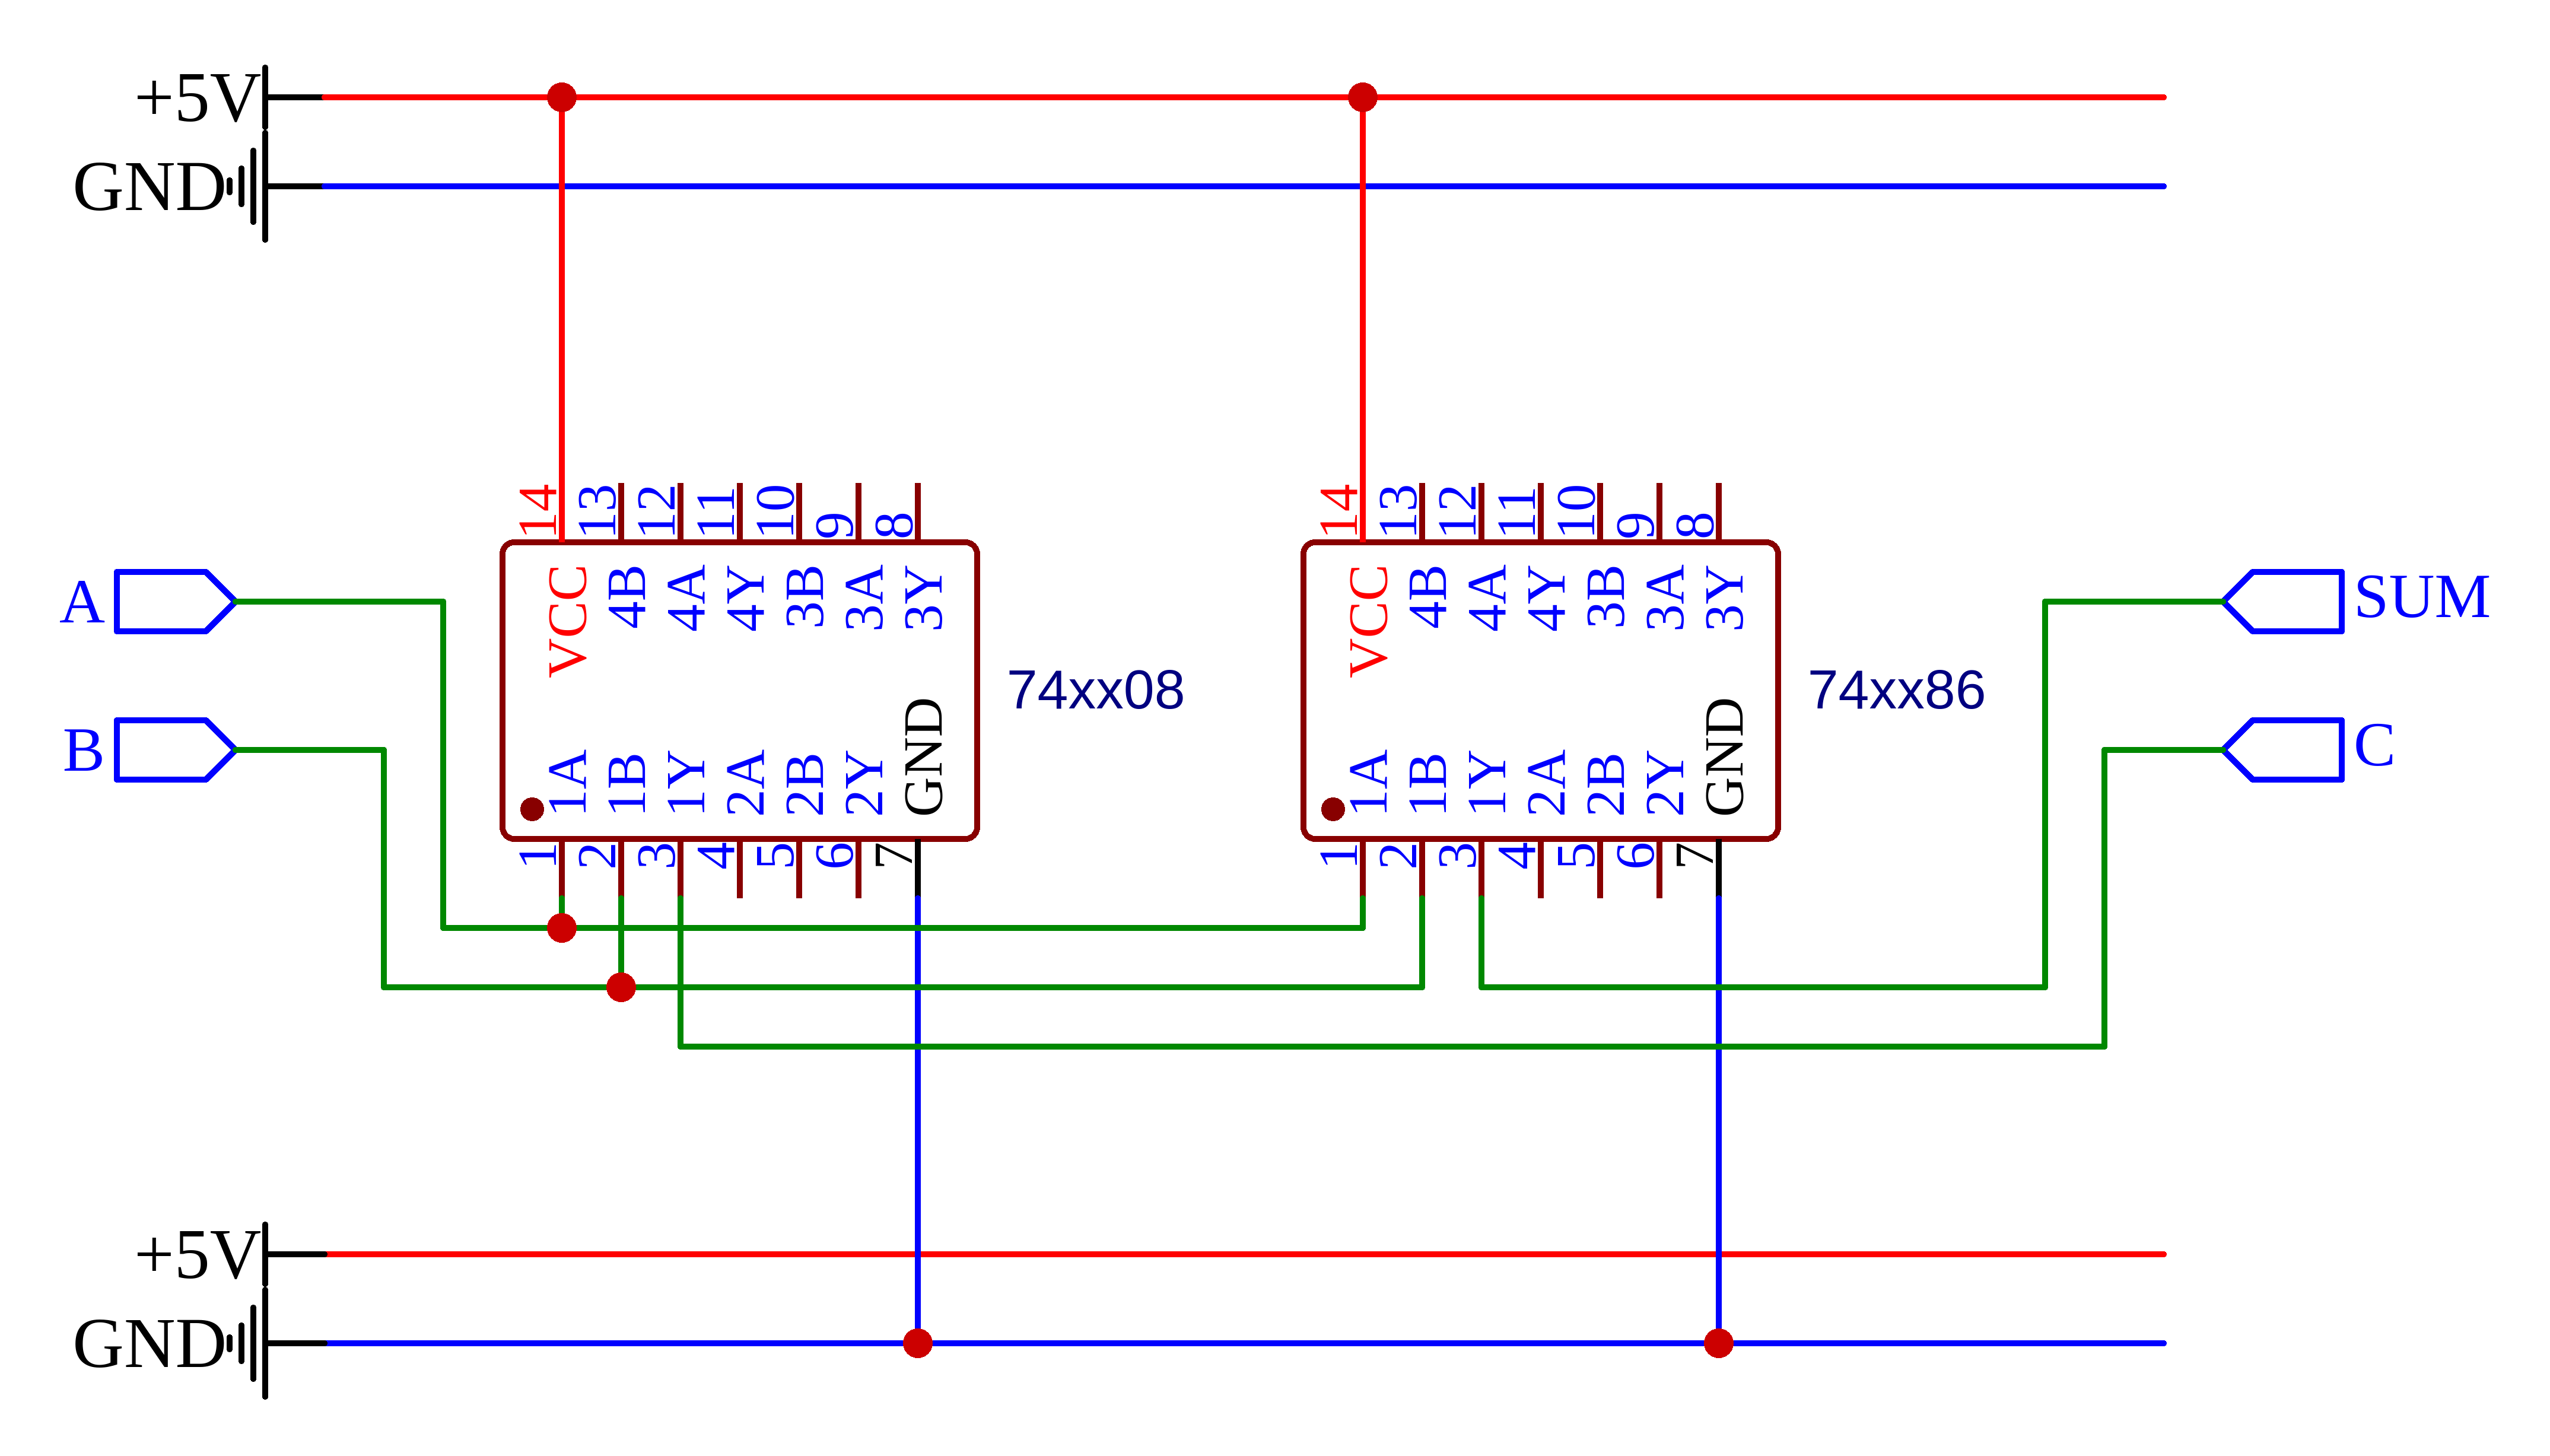
\includegraphics[width=0.8\textwidth]{half_adder_easyeda.png}
	\subcaption{Design in EasyEDA}
\end{subfigure}
\caption{Half adder design}
\end{figure}

\newpage

\subsubsection{Experiment - Part 2}
In this part, it is required to build a full-adder by adding more gates to the previous part's circuit. There is one additional input, \emph{carry in}, but the number of outputs remains the same. The function we are interested in is given in Fig. 2a. The outputs are the same as in half-adder if \emph{carry in} is zero, but when it is one, the outputs are incremented. What happens is in fact two additions, which can be done with a trick by putting another copy of half adder and an OR gate, as shown in Fig. 2b. Therefore, in the experiment, the half-adder from the previous part was not disassembled. Fig. 2c contains the same ICs plus an OR gate ($74xx32$), with denser wiring.
\begin{figure}[H]
\begin{subfigure}{0.3\textwidth}
\centering
\begin{tabular}{|c|c|c|c|c|}
\hline
A &	B & C$_{IN}$ & SUM & C$_{OUT}$ \\
\hline
0 & 0 & 0 & 0 & 0 \\
0 & 0 & 1 & 1 & 0 \\
0 & 1 & 0 & 1 & 0 \\
0 & 1 & 1 & 0 & 1 \\
1 & 0 & 0 & 1 & 0 \\
1 & 0 & 1 & 0 & 1 \\
1 & 1 & 0 & 0 & 0 \\
1 & 1 & 1 & 1 & 0 \\
\hline
\end{tabular}
\subcaption{Truth table}
\end{subfigure}%
\hspace{1em}%
\begin{subfigure}{0.7\textwidth}
\centering
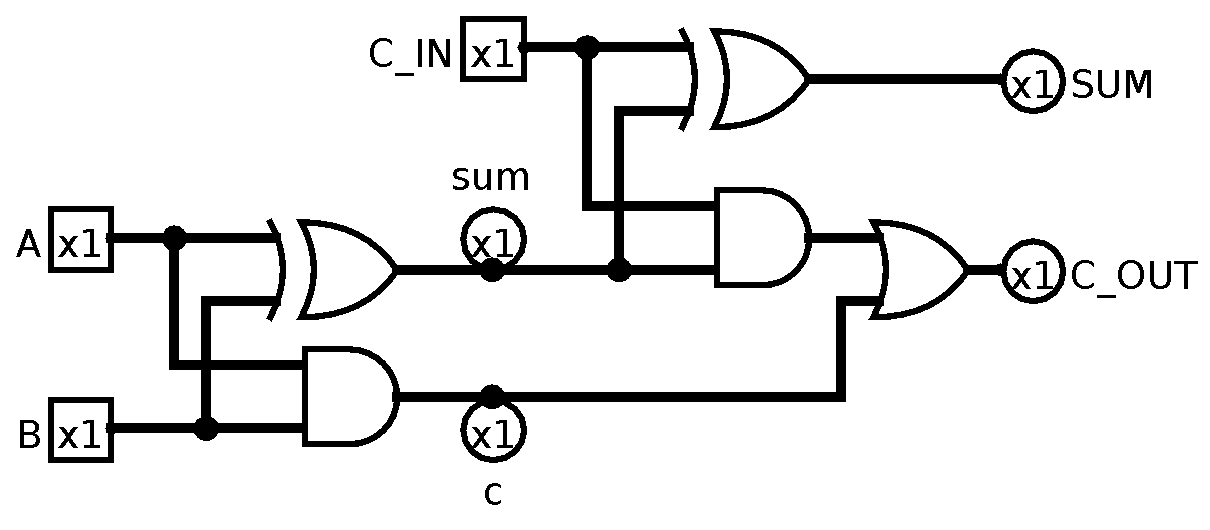
\includegraphics[width=\textwidth]{full_adder_logisim.png}
\subcaption{Design in Logisim}
\end{subfigure}
\begin{subfigure}{\textwidth}
	\centering
	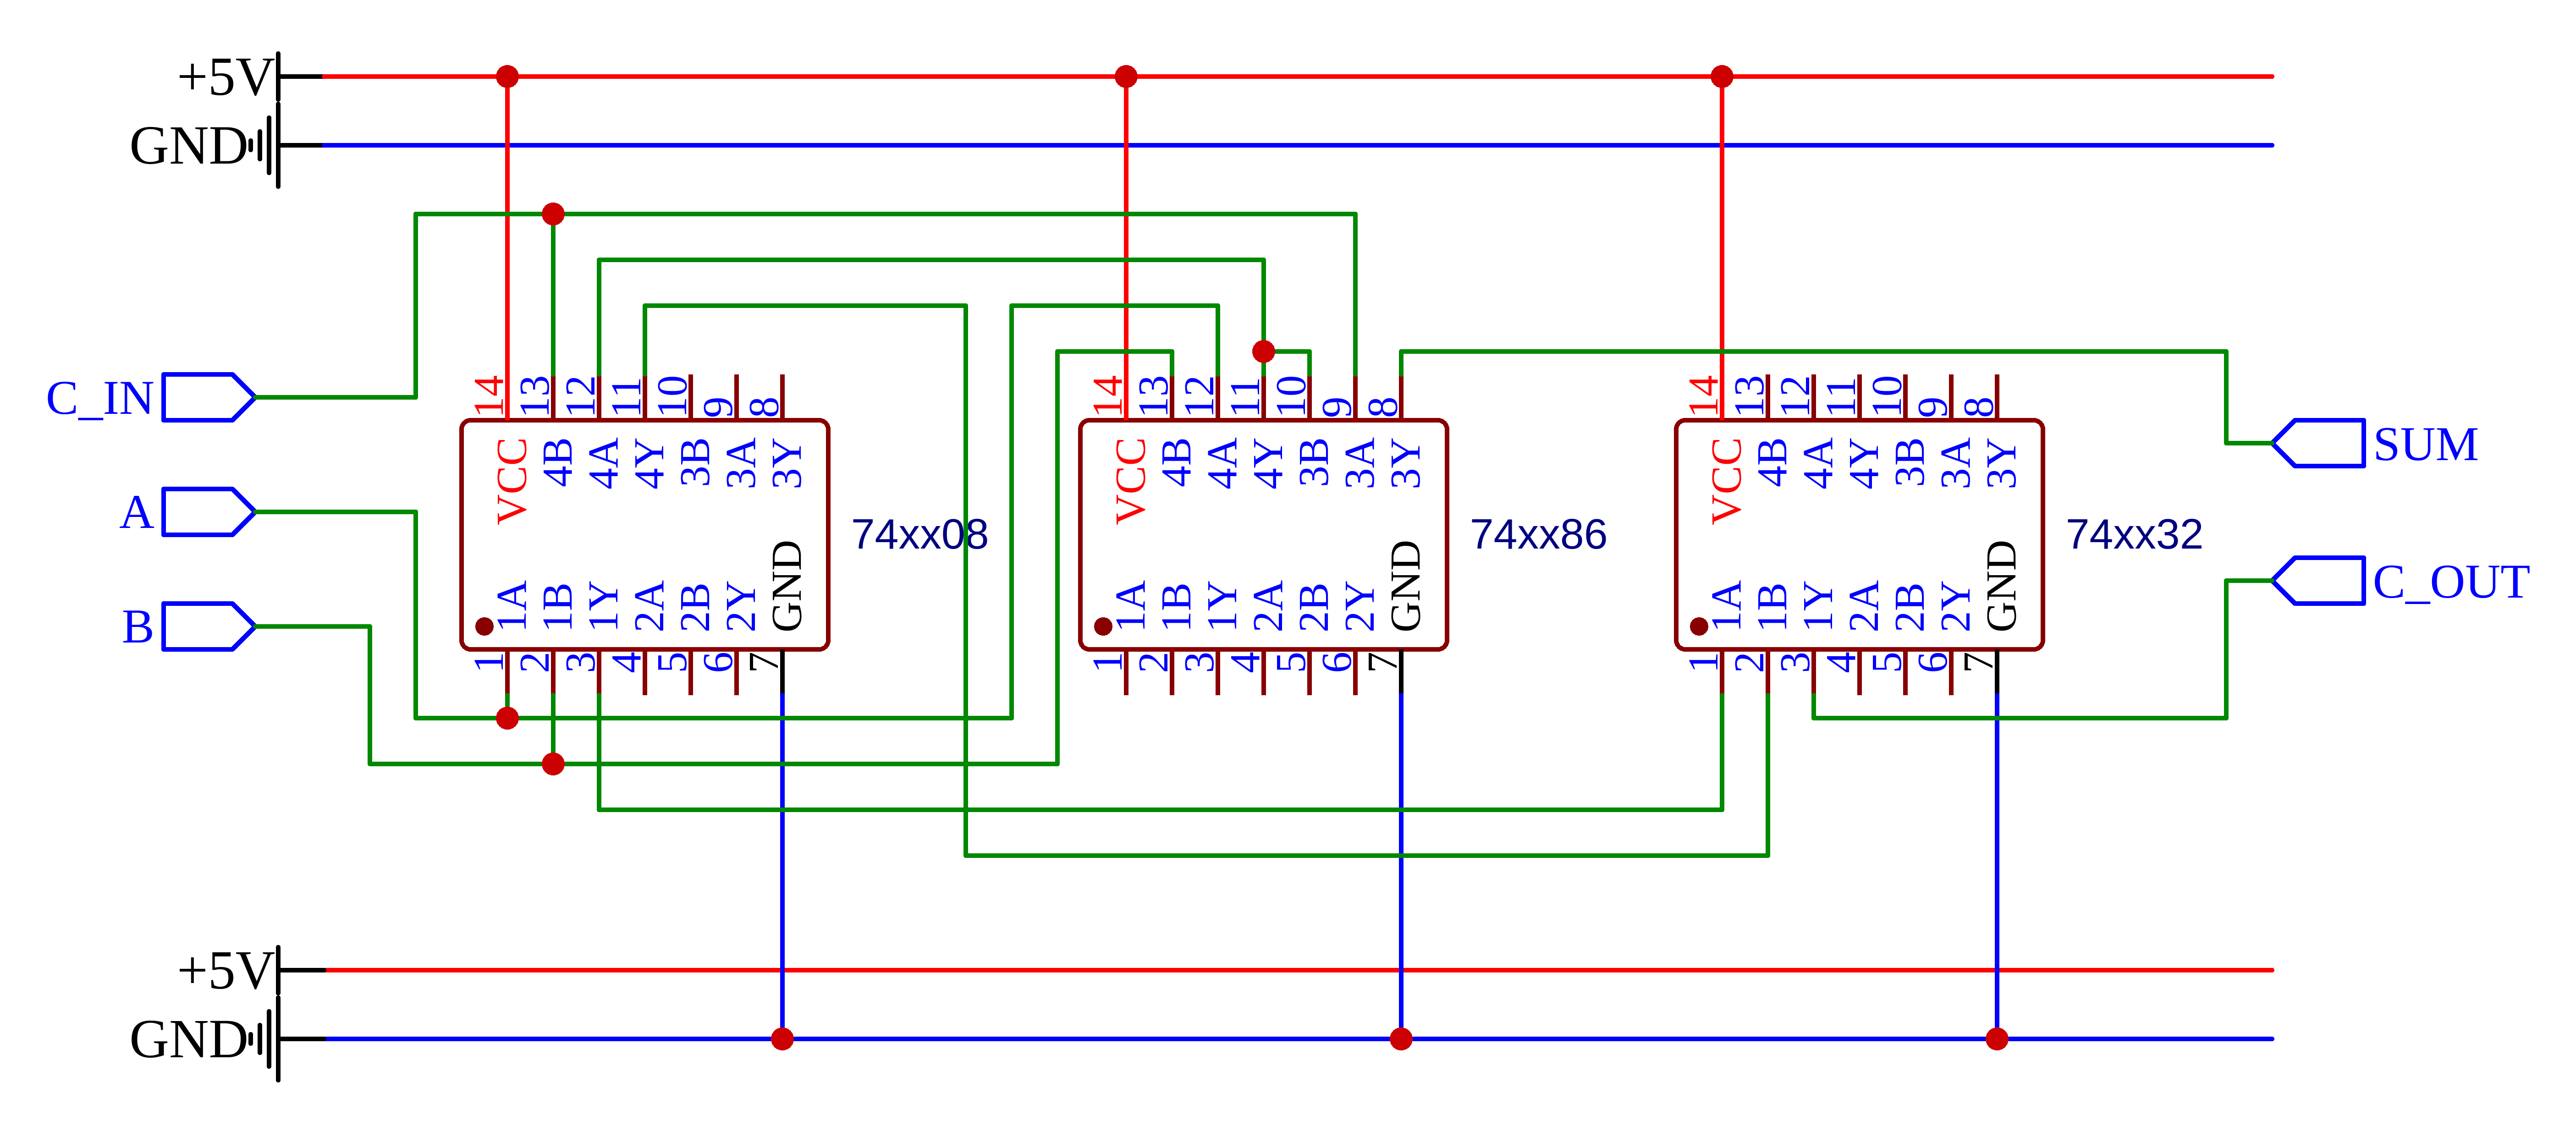
\includegraphics[width=\textwidth]{full_adder_easyeda.png}
	\subcaption{Design in EasyEDA}
\end{subfigure}
\caption{Full adder design as extension of a half adder}
\end{figure}

\newpage

\subsubsection{Experiment - Part 3}
In this part, a four-bit full adder integrated circuit ($74xx83$) was used to add and subtract two four-bit numbers. To select between addition and subtraction, XOR gates ($74xx86$) were used as shown in the following diagram:
\begin{figure}[H]
	\centering
	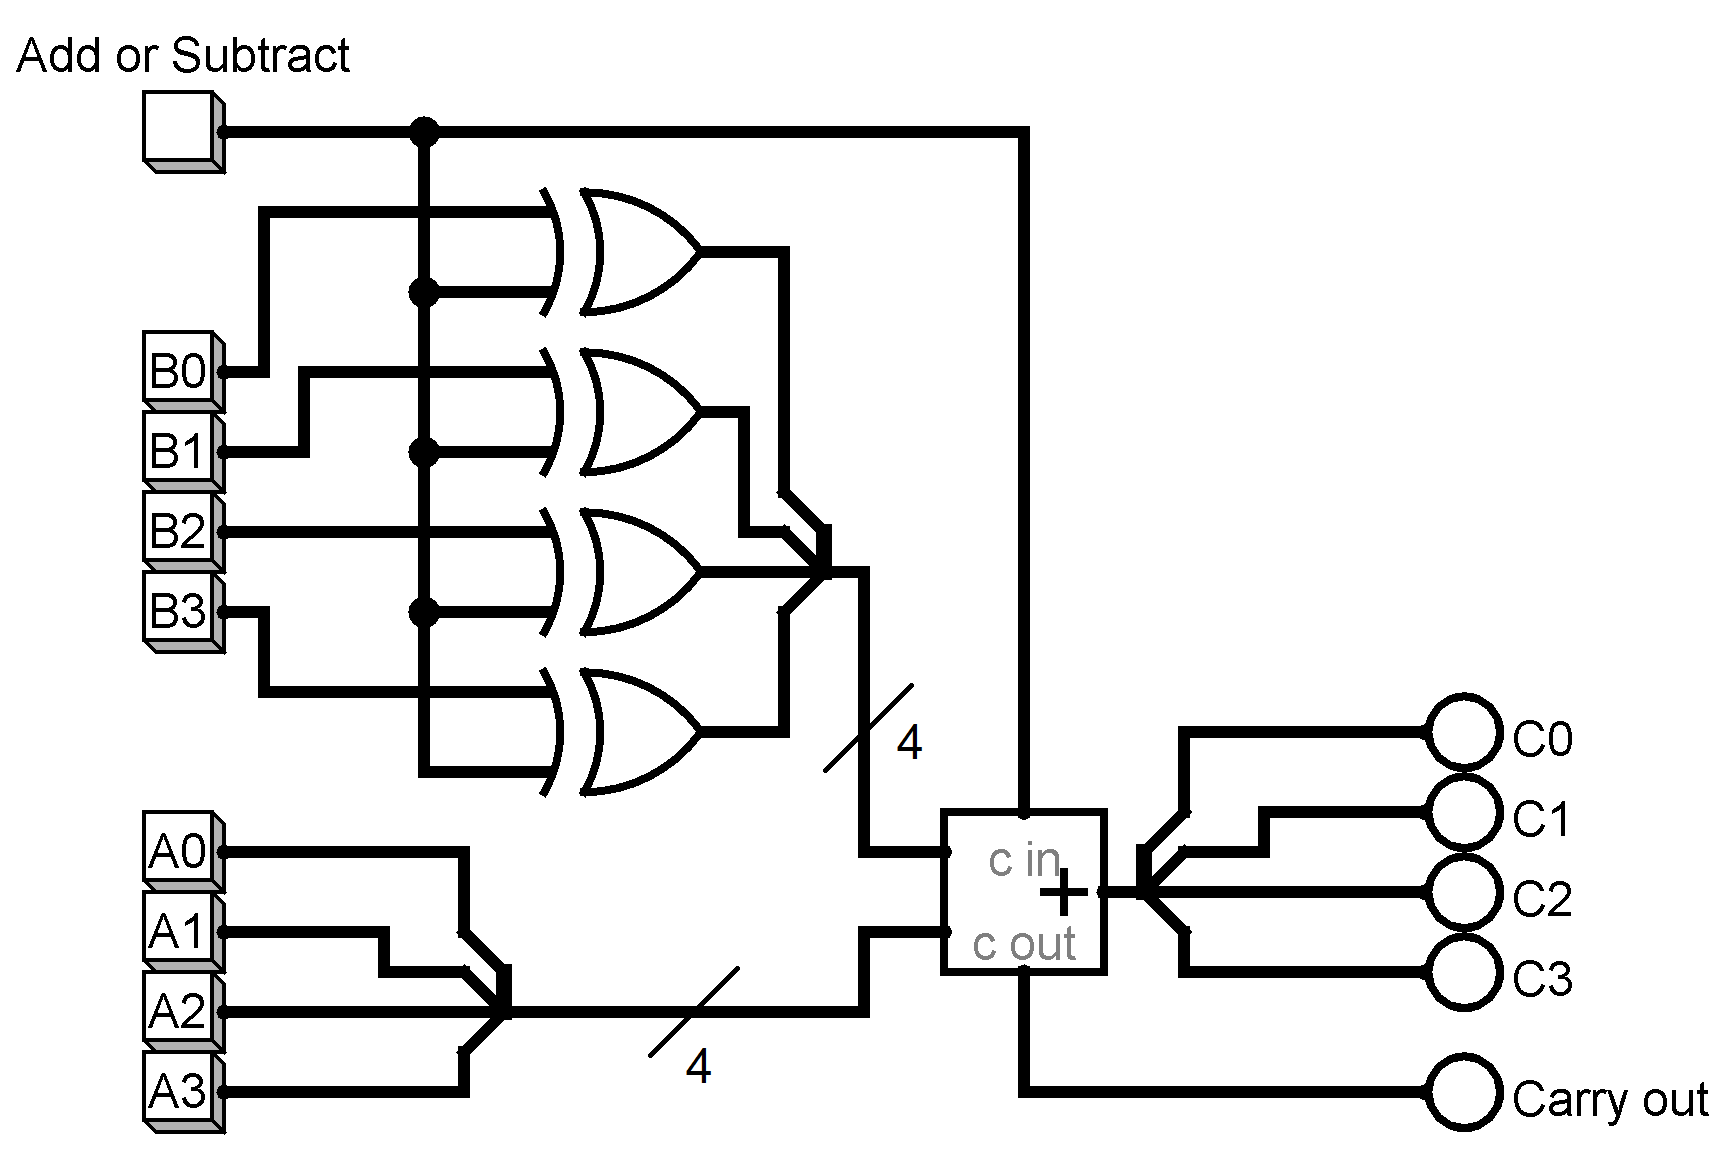
\includegraphics[width=0.6\textwidth]{part3.png}
	\caption{Four-bit adder-subtractor}
\end{figure}

A couple of inputs were tested with addition and subtraction, and the results were interpreted as signed and unsigned:

\begin{figure}[H]
\centering
\begin{tabular}{|c|c|c|c|c|}
\hline
A & B & Carry & Result in Binary & Result in Decimal \\
\hline
0101 & 0111 & 0 & 1100 & +12 \\
1101 & 1001 & 1 & 0110 & +6 \\
1111 & 1111 & 1 & 1110 & +14 \\
0110 & 1101 & 1 & 0011 & +3 \\
\hline
\end{tabular}
\caption{Unsinged A + B computation results}
\end{figure}

\begin{figure}[H]
\centering
\begin{tabular}{|c|c|c|c|c|c|}
\hline
A & B & Overflow & Result sign & Result in Binary & Result in Decimal \\
\hline
0101 & 0111 & yes & $-$ & 1100 & $-4$ \\
1101 & 1001 & yes & + & 0110 & +6 \\
1111 & 1111 & no & $-$ & 1110 & $-2$ \\
0110 & 1101 & no & + & 0011 & +3 \\
\hline
\end{tabular}
\caption{Signed A + B computation results}
\end{figure}

\begin{figure}[H]
\centering
\begin{tabular}{|c|c|c|c|c|}
\hline
A & B & Borrow & Result in Binary & Result in Decimal \\
\hline
0101 & 0111 & yes & 1110 & +14 \\
1101 & 1001 & no & 0100 & +4 \\
1111 & 1111 & no & 0000 & 0 \\
0110 & 1101 & yes & 1001 & +9 \\
\hline
\end{tabular}
\caption{Unsinged A - B computation results}
\end{figure}

\begin{figure}[H]
\centering
\begin{tabular}{|c|c|c|c|c|c|}
\hline
A & B & Overflow & Result sign & Result in Binary & Result in Decimal \\
\hline
0101 & 0111 & no & $-$ & 1110 & $-2$ \\
1101 & 1001 & no & + & 0100 & +4 \\
1111 & 1111 & no & + & 0000 & 0 \\
0110 & 1101 & yes & $-$ & 1001 & $-7$ \\
\hline
\end{tabular}
\caption{Signed A - B computation results}
\end{figure}

\section{DISCUSSION}
During the experiment, we once again practiced wiring logic series integrated circuits according to gate circuit diagrams. This is not always a trivial task, given the pinout and package shape of integrated circuits. We learned a new way of creating a full-adder, by using two half-adders, instead of calculating and simplyfing a complicated expression. Perhaps, the full-adder could have been implemented using fewer gates; however, sometimes it is better to trade-off number of gates with reusability of a ready circuit. In the last part, we saw that the results of binary arithmetic operations can be interpreted in different ways. Sometimes it creates ambiguity, and in large systems one could prefer using signed notation only, because signed numbers include both positive and negative values. Also, modern processors offer resources enough to never run into problems such as carry, borrow and overflow. However, no matter the capabilities of the system, if the hardware and software designers know what they are doing, they can optimize size of registers, number of gates, flag checks, etc.

\section{CONCLUSION}
In conclusion, knowing how adder circuits work internally is an important thing, but using dedicated chips is far more practical. Even though in the last part we had a full-adder ready in a dual in-line package, which saved a lot of space and wires, connecting inputs and outputs was still a challange and error-prone. We managed to distinguish between the input A, input B and output by using specific colors for wires. Even so, we accidentally connected the bits of input A in the reverse order, which caused a lot of confusion at first. Nonetheless, we managed to push the integrated circuits to the limit, without leaving any unused functionality.


\end{document}